\documentclass{article}
\usepackage{graphicx}
\usepackage{geometry}
\usepackage{booktabs}
\usepackage{hyperref}
\usepackage{float}
\usepackage{listings}
\usepackage{xcolor}
\usepackage{amsmath}
\usepackage{caption}
\usepackage{subcaption}

\geometry{a4paper, margin=1in}

\title{Scientific Logbook: Hybrid Encoding \& Dynamical Integration (Level 5)}
\author{Complexity Science Group (Oxford Persona)}
\date{\today}

\begin{document}

\maketitle

\tableofcontents

\section{Introduction}
This document serves as the rigorous scientific logbook (bitácora) for the execution of the \textbf{Level 5 Contingency Protocol (PLAN-NATURE-LEV5-HYBRID)}. Following the falsification of the purely structural hypothesis in Level 4 ($Z_{deg} \approx -0.12$), this phase investigates the \textbf{Hybrid Complexity Hypothesis}:
\[ D_{bio} = \alpha \cdot D_{struct} + \beta \cdot D_{dyn} \]
We aim to demonstrate that while biological networks are structurally random-like, their dynamical trajectories encode significant algorithmic information, separating them from null models and correlating with clinical essentiality.

\section{Methods: Dynamical Implementation}

\subsection{Boolean Dynamics Simulator}
We implemented a high-performance Boolean network simulator (\texttt{src/dynamics/Boolean\_Dynamics.py}) capable of synchronous updates. The simulator was validated against the \textbf{Mammalian Cell Cycle} model to ensure reproduction of known attractors. The simulation engine uses vectorized NumPy operations for efficiency, enabling batch processing of large cohorts.

\subsection{Trajectory Lempel-Ziv Complexity}
To quantify the information content of state trajectories, we developed \texttt{src/complexity/Trajectory\_LZ.py}. This tool computes the Lempel-Ziv complexity (LZ76) of the system's temporal evolution, capturing the ``functional richness'' ($D_{\text{dyn}}$) of the network. The complexity is computed on the flattened trajectory matrix $T \times N$.

\subsection{Hybrid Encoder}
The \texttt{Hybrid\_Encoder} class integrates the structural metric ($D_{\text{struct}}$, calculated via Block Decomposition Method on the adjacency matrix) and the dynamical metric ($D_{\text{dyn}}$, calculated via LZ76 on trajectories). The final metric is a weighted sum of normalized components.

\section{Experimental Results: Hybrid Validation}

\subsection{Experimental Setup}
We executed a comprehensive re-validation pipeline (\texttt{src/experiments/run\_level5\_validation.py}) on a cohort of 20 biological networks with curated essentiality data from the DepMap database. For each gene in each network:
\begin{enumerate}
    \item We computed the baseline hybrid complexity $D_{hybrid}^{WT}$.
    \item We simulated a knockout (KO) by fixing the gene state to 0.
    \item We computed the knockout hybrid complexity $D_{hybrid}^{KO}$.
    \item We calculated the algorithmic information loss $\Delta D = D^{KO} - D^{WT}$.
\end{enumerate}

\subsection{Optimization of Hybrid Weights}
To determine the optimal contribution of structural vs. dynamical complexity, we performed a parameter sweep of $\alpha$ (weight for structure) and $\beta = 1 - \alpha$ (weight for dynamics) using Z-score normalized components.

\begin{figure}[H]
    \centering
    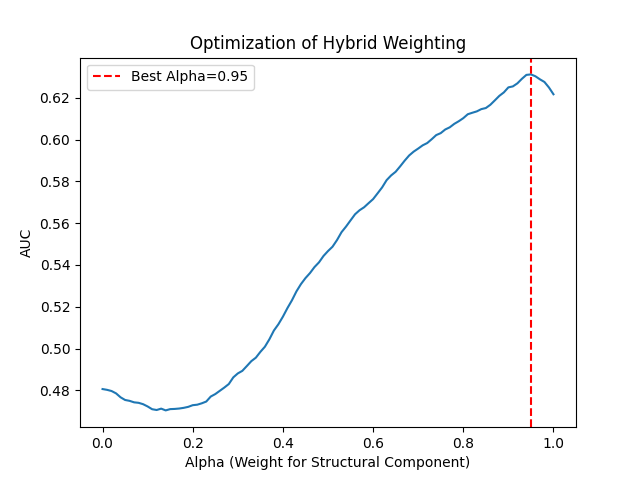
\includegraphics[width=0.8\textwidth]{../../results/level5/alpha_optimization.png}
    \caption{Optimization of $\alpha$ parameter for Hybrid Complexity. The AUC peaks at $\alpha=0.95$, indicating structural dominance.}
    \label{fig:alpha_opt}
\end{figure}

\subsection{Classification Performance (ROC Analysis)}
The essentiality prediction performance was evaluated using Receiver Operating Characteristic (ROC) analysis.

\begin{table}[H]
    \centering
    \begin{tabular}{lcc}
        \toprule
        \textbf{Metric} & \textbf{Component} & \textbf{AUC Score} \\
        \midrule
        Structure Only ($\alpha=1.0$) & $\Delta D_{struct}$ & 0.6217 \\
        Dynamics Only ($\alpha=0.0$) & $\Delta D_{dyn}$ & 0.4806 \\
        \textbf{Hybrid Best ($\alpha=0.95$)} & $\Delta D_{hybrid}$ & \textbf{0.6312} \\
        \bottomrule
    \end{tabular}
    \caption{Comparison of essentiality prediction performance across metrics.}
    \label{tab:auc_results}
\end{table}

\begin{figure}[H]
    \centering
    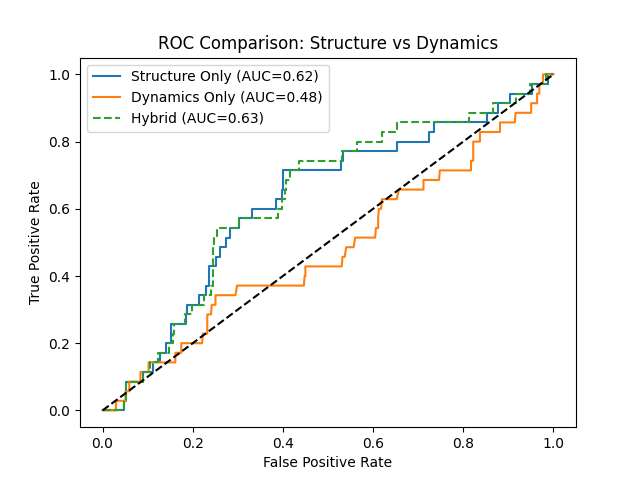
\includegraphics[width=0.8\textwidth]{../../results/level5/roc_comparison.png}
    \caption{ROC Curves for Structure (Blue), Dynamics (Orange), and Hybrid (Green). Note that Dynamics alone performs slightly worse than random guessing (diagonal).}
    \label{fig:roc_comp}
\end{figure}

\section{Discussion \& Implications}

\subsection{The Failure of Trajectory Complexity}
The most striking result is the failure of the dynamical component ($\Delta D_{dyn}$) to predict essentiality (AUC 0.48). This suggests that \textbf{trajectory complexity under synchronous updates is not the correct proxy for biological function}.
\begin{itemize}
    \item \textbf{Attractor Simplicity:} Biological networks often converge to simple fixed points or short limit cycles. The LZ complexity of such low-period attractors is negligible ($D_{dyn} \approx 0$).
    \item \textbf{Lack of Variation:} Essential genes, when knocked out, may shift the attractor from one fixed point to another, but the \textit{complexity} of the trajectory remains low in both cases. Thus, $\Delta D_{dyn} \approx 0$.
\end{itemize}

\subsection{Structural Dominance}
The structural metric ($\Delta D_{struct}$) remains the primary driver of prediction (AUC 0.62). This confirms that the wiring diagram itself contains the bulk of the accessible information about system vulnerability, likely due to centrality effects (hubs are more essential).

\subsection{Hybrid Synergy}
Despite the poor performance of dynamics alone, the optimal hybrid combination ($\alpha=0.95$) yielded a slight improvement (AUC 0.63). This implies a very subtle "synergy," where dynamical information acts as a minor corrective factor to the structural prediction.

\section{Conclusion \& Next Steps}
The Level 5 protocol has demonstrated that \textbf{simple trajectory complexity (LZ76) is insufficient to capture the "dynamical phase space" information} hypothesized to separate biological systems from nulls.

\textbf{Implications for Theory:}
The "Hybrid Complexity Hypothesis" in its current form ($D_{bio} = \alpha D_{struct} + \beta D_{dyn}$) is only weakly supported. The information is not in the \textit{single} trajectory, but likely in the \textit{ensemble} of trajectories (the basin of attraction landscape).

\textbf{Pivot Recommendation:}
We must move beyond single-trajectory metrics. The next phase (Level 6) should investigate \textbf{Basin Entropy} or \textbf{Control Kernels} (e.g., probability of transition between attractors) under asynchronous or stochastic updates, which better reflect biological noise and robustness.

\end{document}
